% !TEX encoding = UTF-8
% !TEX program = pdflatex
% !TEX root = InformationRetrieval.tex
% !TEX spellcheck = it-IT

% 13 Ottobre 2016

%section indicizzazione
%subsection fasi del processo di indicizzazione
%subsubsection Stemming

\paragraph{Dictionary-based stemmer}

Un modo per risolvere questi problemi è quello di basarsi su degli elenchi di parole preparati da degli esperti di linguistica.

Questi dizionari possono essere utilizzati ad esempio per riconoscere che \textit{is, be} e \textit{was} sono tutte forme dello stesso verbo.

C'è però un problema con l'aggiornamento del dizionario, perché nella lingua naturale vengono aggiunte in continuazione nuove parole.
Si può quindi creare il dizionario in modo automatico effettuando un'analisi statistica dei testi del documento, oppure si può scegliere di utilizzare in modo combinato uno stemmer algoritmico e uno basato su dizionario.

\subsubsection{Fase 4: Composizione dei termini}

In alcuni contesti può essere importante ricostruire alcune frasi o termini, come nella ricerca dei documenti scritti da una determinata persona.
Inoltre la maggior parte delle query effettuate dagli utenti sono costituite da varie parole e in alcuni casi questo insieme deve essere considerato come una frase.

Volendo questa fase può essere fatta subito dopo l'analisi lessicale, ma le informazioni che vengono estratte dalle altre fasi può aiutare ad effettuare una composizione migliore.
Infatti si può scegliere di effettuare la composizione delle frasi sia utilizzando le parole originali che con gli stem.

L'analisi e la ricostruzione delle frasi è computazionalmente onerosa, pertanto il problema è stato studiato molto e i risultati che si sono ottenuti sono utilizzabili per raggiungere obiettivi specifici di realizzazione di un IRS.

Il come e quando ricostruire le frasi e le relative conseguenze dipendono molto dal modello che viene utilizzato, pertanto l'argomento verrà trattato più avanti.

\subsubsection{Fase 5: Creazione dell'indice}

Il modo più semplice di costruire l'indice è quello di utilizzare una matrice binaria che ha come righe le parole o gli stem, come colonne i vari documenti e in una determinata cella viene messo un 1 solo se la parola compare nel documento.
Così facendo però non viene tenuto conto della frequenza e del contenuto informativo della parola, inoltre non è possibile trovare un modo per ordinare i risultati della ricerca.

\begin{figure}[ht]
\centering
\begin{minipage}[b]{0.45\linewidth}
		\centering
  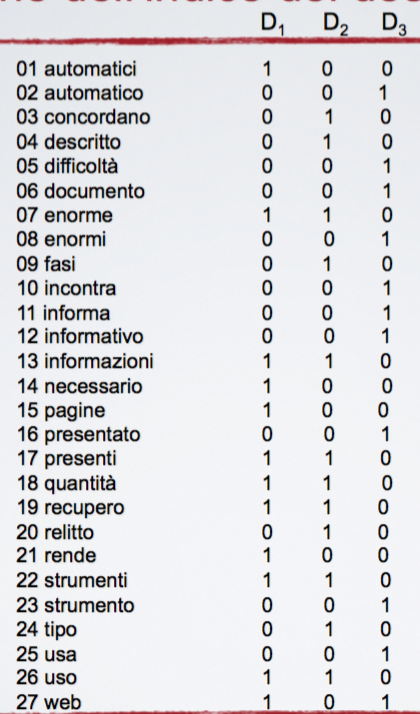
\includegraphics[width=0.7\linewidth]{images/l5-index-1}
  \caption{Indice delle parole}

\end{minipage}
\quad
\begin{minipage}[b]{0.45\linewidth}
	\centering
  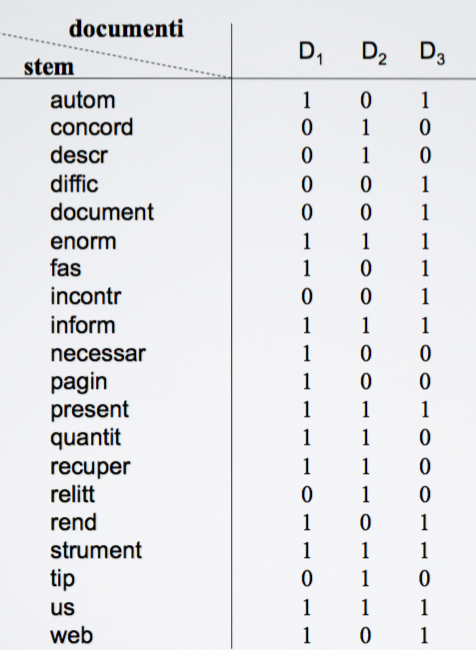
\includegraphics[width=0.7\linewidth]{images/l5-index-2}
  \caption{Indice degli stem. Ci sono dei casi in cui uno stem compare in tutti i documenti}
\end{minipage}
\end{figure}

Per risolvere questi problemi si posso utilizzare dei pesi per le varie parole, che vengono assegnati con una \textbf{funzione di pesatura} la quale può essere:

\begin{itemize}
	\item \textbf{Binaria}: se tiene conto solamente della presenza o meno della parola.
	\item \textbf{In base alla frequenza}: se considera il numero di occorrenze delle parole nei documenti e nella collezione.
\end{itemize}

\begin{figure}[htbp]
	\centering
	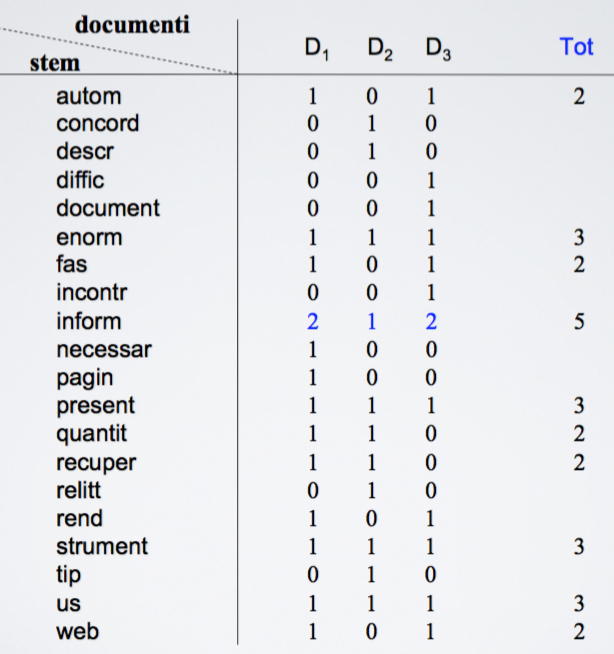
\includegraphics[width=0.4\linewidth]{images/l5-index-3}
	\caption{Indice degli stem che prende in considerazione anche le frequenze}
	\label{fig:l5-index-3}
\end{figure}


La pesatura può assegnare a ciascuno termine la frequenza di occorrenza del termine in un documento (\textbf{Term Frequency}) oppure la frequenza di occorrenza del termine all'interno della collezione (\textbf{Inverse Document Frequency}). Entrambi gli schemi verranno approfonditi più avanti.

Tipicamente nell'indice vengono memorizzati i dati grezzi, ovvero la frequenza assoluta, per calcolare i pesi in fase di reperimento, questo perché se l'indice contenesse direttamente i pesi, all'aggiunta di un nuovo documento sarebbe necessario andare a ricalcolare tutti i pesi di tutti i documenti. Un altro motivo è dato dal fatto che il peso serve solo per le parole che compaiono all'interno della query e quindi il calcolo non è oneroso e può essere fatto online.

L'indice finale dei descrittori è tipicamente una matrice sparsa molto grande e quindi è necessario utilizzare delle apposite strutture dati per memorizzare i dati.
Tipicamente viene utilizzato un \textbf{posting file} (o \textbf{inverted index}) che contiene la lista delle parole e per ogni parola è presente una lista di coppie, ognuna delle quali contiene l'identificativo del documento e la frequenza assoluta della parola all'interno del documento.

\begin{figure}[htbp]
	\centering
	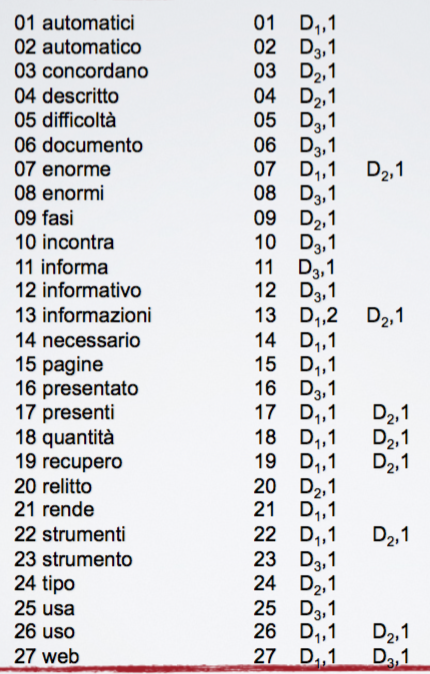
\includegraphics[width=0.3\linewidth]{images/l5-index-4}
	\caption{Esempio di posting file}
\end{figure}

\textbf{{\color{Red} Possibile esercizio:}} Dati dei documenti testuali si effettui la loro indicizzazione automatica creando l'indice dei descrittori. Si descriva una possibile strategia per la costruzione di una stop-list corrispondente ai documenti forniti.

\section{Ranking}

L'approccio base è quello di fornire una lista di documenti ordinata a partire dai dati presenti nell'indice.
Ma non sempre questo va bene:
\begin{itemize}
\item Due utenti possono effettuare la stessa query anche se hanno esigenze informative diverse.
\item Alcuni utenti filtrano la lista, non sempre si concentrano sul primo risultato, ma guardano anche altre cose, come lo snippet fornito nella SERP di Google.
\end{itemize}

Si può quindi pensare di creare un sistema di ranking che si basa su altre risorse, tipicamente sul machine learning, per creare un ordinamento migliore e che tiene conto delle caratteristiche degli utenti.

Quindi l'idea è quella di fare un primo ranking tenendo conto degli indici del sistema e poi ristrutturarlo utilizzando altre tecniche.
